\section{Rule and Example Generation} \label{sec:rules_gen}
%This and the following Section are the main technical contributions of the paper. 
In this Section we describe how to generate the universe of all possible rules. 
%, while in the next Section we propose a greedy approximated solution to our problem. %weighted set cover problem.
%In this Section 
We start by assuming that the positive and the negative examples are given, and then show how they can be computed. However, our approach is independent of how $G$ and $V$ are generated: they could be manually crafted by domain experts, with significant additional manual effort.

In the following we discuss the discovery of positive rules, i.e., having true facts in $G$ and false facts in $V$.
In the dual problem of negative rule discovery our approach remains unchanged, we just switch the roles of $G$ and $V$. The generation set $G$ is formed out of negative examples (false facts), while the validation set $V$ is built from the set of positive examples (true facts). 
%Now it should be more clear why we introduced the second constraint of LCWA on predicates. 
%THIS CAN/SHOULD BE AT BEGINNING OF SEC 3 <<<<<<<<<<
%A crucial role in our approach is played by the two input sets $G$ and $V$, used to generate and validate rules. We will show that discovering negative rules is the dual problem of discovering positive rules, therefore we assume to be in the setting of generating positive rules.
%We will explain how to switch to the negative setting at the end of this section. % DO WE???? <<<<<


\vspace{-1ex}	
\subsection{Rule Generation} \label{sec:rules_generation}
\vspace{-1ex}	
%	THIS SHOULD BE WHEN WE ADDRESS THE INCREMENTAL GENERATION %%%%%%%%%%%
%The number of possible rules increases exponentially with the size of the KB and enumerating all of them leads to exploring a huge search space. 
%While loading the KB in memory alleviates this problem~\cite{galarraga2015fast,Chen:2016}, KBs can exceed the size of hundreds of GBs, making a memory-based solution infeasible without significant hardware, such as a distributed platform~\cite{Chen:2016,DBLP:conf/sigmod/FaridRIHC16}. On the contrary, our rule generation technique inspects only a portion of the KB without losing any rule that is good w.r.t. our weighting scheme. Also, since we load only a small fraction of the database into main memory, we can afford a more expressive language compared to previous works. %One could argue that reducing the search space may lead to missing some meaningful rules. 
%%%%%%%%%%%%%%%%%%%%%%%%%

%In our approach, 
%The first task we address is the generation of 
In the universe of all possible rules $R$, 
each rule must cover one or more examples from the generation set $G$. 
Thus the universe of all possible rules is generated by inspecting the elements of $G$ alone. 
%In fact, a rule that does not cover any element of $G$ will never be part of the optimal solution, since it will not give any contribution to the set cover problem. %This is a key part of our generation approach: we do not inspect the entire KB, but only entities belonging to $G$. 
The smaller the size of $G$, the smaller is the search space for rule generation. 
%On the contrary, other KB rule mining approaches search for valid rules by loading and exploring the entire KB~\cite{galarraga2015fast,Chen:2016}. 
%GO TO RELATED
%This is typically done by initially looking at all facts that share a common predicate, and then expanding these facts with other predicates that share common entities~\cite{galarraga2015fast} (TODO : CITE Ontological path finding). 
%Alternatively other approaches leverage on well established relational database techniques such as functional dependencies discovery (TODO: cite SIGMOD DEMO Data Lakes). 

%This is the main reason why previous approaches solve the problem by loading the entire KB into main memory and by aggresively indexing triples on subject, object, and predicate. 
%We will show in Section~\ref{sec:krd_comparative} that our generation technique for $G$ creates a representative (reduced) view of the entire search space.

\begin{figure}[t]
	\centering
	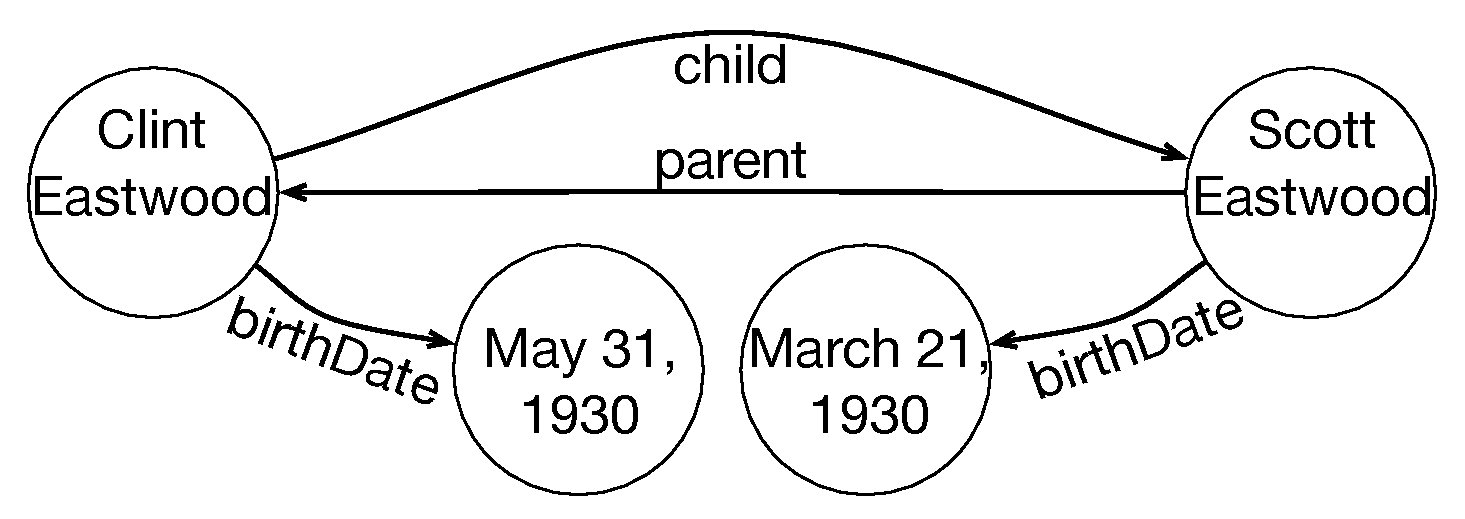
\includegraphics[width=0.8\columnwidth]{include/figure/graph_example.pdf}
	\vspace{-1ex}
	\caption{Graph example of \dbpedia for four triples.}
	\label{fig:krd_graph_example}
	\vspace{-3ex}
\end{figure}

%The data structure \krd leverages on is a straightforward translation of 
We translate a KB $\kb$ into a directed graph: entities and literals are the nodes, and there is a directed edge from node $a$ to node $b$ for each triple $\<a,rel,b\> \in \kb$. 
%IS THIS NOTATION NEW HERE???
Edges are labelled with the relation $rel$ that connects subject to object. Figure~\ref{fig:krd_graph_example} shows a portion of \dbpedia~\cite{bizer2009dbpedia} for four triples.
%that connects two person in child and parent relationships, along with their dates of birth. The graph represents information for four KB triples.
%(two birth dates, one parent, and one child relation).

The body of a rule can be seen as a path in the graph. In Figure~\ref{fig:krd_graph_example}, the body $\atom{child}{a}{b} \wedge \atom{parent}{b}{a}$ corresponds to the path \textit{Clint Eastwood} $\rightarrow$ \textit{Scott Eastwood} $\rightarrow$ \textit{Clint Eastwood}. 
As introduced in Section~\ref{sec:krd_language}, a valid body of a rule contains target variables $a$ and $b$ at least once, every other variable at least twice, and atoms are transitively connected. 
If we allow navigation of edges independently of the edge direction, we can translate bodies of valid rules to valid paths on the graph.
\begin{inparaenum}[(i)]
	Given a pair of entities $(x,y)$, a {\em valid body} corresponds to a valid path $p$ on the graph such that:
	\item $p$ starts at the node $x$;
	\item $p$ covers $y$ at least once;
	\item $p$ ends in $x$, in $y$, or in a different node that has been already visited.
\end{inparaenum}
%I DONT SEE CLEARLY THE TRANSLATION HERE, WHY IT HAS TO END in one of those? I would rather expect as third : p covers an incoming and out coming edge for each node different from x and y  %%%%%%%<<<<<<<<<<<<<<<
%NOT ESSENTIAL
%The transitive connection between atoms is always guaranteed by the construction property of a path $p$: for each node $n$ in $p$ there always exists a subpath that connects $n$ to every other node in $p$.
%
%In other words, 
Given the body of a rule $r_{body}$, $r_{body}$ covers a pair of entities $(x,y)$ iff there exists a valid path on the graph that corresponds to $r_{body}$. This implies that for a pair of entities $(x,y)$, we can generate bodies of all possible valid rules by computing all valid paths from $x$ to $y$ (and vice versa) with a standard BFS. The key point is the ability to navigate each edge in any direction by turning the original directed graph into an undirected one.
%is the VICE VERSA CORRECT?? <<<<
%Despite the navigation over an undirected graph
However, we need to keep track of the original direction of the edges. This is essential while translating paths to rule bodies. In fact, %if we navigate an edge \texttt{rel} between $a$ and $b$, going 
an edge directed from $a$ to $b$ produces the atom $\atom{rel}{a}{b}$, while $b$ to $a$ produces $\atom{rel}{b}{a}$. 
%The two atoms are different, as the facts exist in the KB only wrt the original direction of the edge (determined by the position of the variables).
%NOTICE A FEW CHANGES IN WORDING HERE

Since every node can be traversed multiple times, for two entities $x$ and $y$ there might exist infinite valid paths starting from $x$. This is avoided with a $maxPathLen$ parameter that constrains the search space by determining the maximum number of edges in the path. When translating paths to Horn Rules, $maxPathLen$ is the maximum number of atoms allowed in the body of the rule.
We will validate the use of this parameter in Section~\ref{sec:krd_experiments}. 
%This parameter is essential 
%to avoid the discovery of rules with infinite body length and 
%to constraint the search space.
We now describe the two main steps in our generation of the universe of all possible rules for $G$. 

\noindent \myparagraph{1. Create Paths}
%The main advantage of inspecting just the generation set $G$ is the capability of loading only a small portion of the graph that is currently needed. 
Given a pair of entities $(x,y)$, we retrieve from the KB all nodes at a distance smaller than $maxPathLen$ from $x$ or $y$, along with their edges. The retrieval is done recursively: we maintain a queue of entities, and for each entity in the queue we execute a SPARQL query against the KB to get all entities (and edges) at distance $1$ from the current entity -- we call these queries \emph{single hop queries}. At the $n$-th step, we add the new found entities to the queue iff they are at a distance less than $maxPathLen-n$ from $x$ or $y$ and they have not been visited before. The queue is initialized with $x$ and $y$. 
%By doing so we retrieve a small portion of the entire KB, the only one needed to discover rules that cover $(x,y)$. 
%We show in the experimental section that SPARQL engines are very fast at executing single hop queries. %DO WE REALLY SHOW IT?? <<<<
%
%\vspace{0.5ex}
%\myparagraph{Navigate Graph}
%The generation of the universe of all possible rules for $G$ is then straightforward: 
%For each element $(x,y) \in G$, we construct the 
Given the graph for every $(x,y)$, we then compute all valid paths starting from every $x$. 

\noindent \myparagraph{2. Evaluate Paths}
Computing paths for every example in $G$ implies also computing the coverage over $G$ for each rule. The {\em coverage} of a rule $r$ is the number of elements in $G$ for which there exists a path corresponding to $r_{body}$. 
%
%do we want to keep the following sentence ?? <<<<<<<<<<<<<<<<<<<<<<<< PAOLO REMOVED ACCORDING TO NEW SEC 3 $$$$$$$$$$$$$<<<<<<
%Our technique also generates single-instance rules: rules that cover only one example $(x,y) \in G$ by instantiating target variables $a$ and $b$ in the rule with $x$ and $y$. 
%
Once the universe of all possible rules has been generated (along with coverages over $G$), computing coverage and unbounded coverage over $V$ requires only the execution of two SPARQL queries against the KB for each rule in the universe (validation queries).
%REDUNDANT 
%We will show in Section~\ref{sec:krd_greedy} how some queries can be avoided, as well as there is no need of enumerating all possible rules in the universe as some of them will never be part of the final solution.

%Clearly, the size of $G$ has a direct impact on the search space and hence on the running time. Since we generate all valid rules for each example in $G$, the search space grows roughly linearly with the size of $G$. If we could know a-priori the minimum subset of examples that lead to the generation of all valid rules, then we could use only those few examples. 
%
%A future direction we are working on exploits exactly this point: how to select a small number of representative examples in order to reduce the size of $G$, without significantly affecting the quality of the output.
%\vspace{-1ex}

One of the goals is to discover more expressive rules. We therefore generate three new atom types as detailed next.

%\vspace{-1ex}
%\vspace{0.5ex}
\noindent \myparagraph{Literal comparison}
In Section~\ref{sec:krd_language} we defined our target language, which, other than predicate atoms, includes literal comparison. 
Their role is to enrich the language with comparisons among literal values other than equalities, such as ``greater than''. 
%or ``less than''. 
To discover such atoms, the graph representation must contain edges that connect literals with one (or more) symbol from $\{<,\leq,\neq,>,\geq\}$. As an example, Figure~\ref{fig:krd_graph_example} should contain an edge `$<$' from node ``\textit{March 31, 1930}'' to node ``\textit{March 21, 1986}". Unfortunately, the original KB does not contain this kind of information, and materializing such edges among all literals is infeasible.

%Once again, the use of a 
The generation set $G$ is the resource point to identify relevant literal comparison.
Since we discover paths for a pair of entities from $G$ in isolation, the size of a graph for a pair of entities is relatively small, thus we can afford to compare all literal values within a single example graph. 
%Since in a single example graph the number of literals is usually small, the creation of a quadratic number of edges w.r.t. the number of literals is affordable. 
%Despite this implies the creation of a quadratic number of edges w.r.t. the number of literals in the graph, within a single example graph the number of literals is usually small thus the quadratic comparison affordable. 
KBs include three types of literals: numbers, dates, and strings. Besides equality comparisons, we add `$>$',`$\geq$',`$<$',`$\leq$' relationships between numbers and dates, and $\neq$ between all literals. These new relationships are treated as normal atoms (edges): $x \geq y$ is equivalent to $\atom{rel}{x}{y}$, where \texttt{rel} is equal to $\geq$. 
%Once we added comparison edges for every input example graph, the discovery of literal comparisons is equivalent to discovering for predicate atoms.

\noindent \myparagraph{Not equal variables}
The ``not equal'' operator introduced for literals is useful for entities as well. 
Consider the rule:
$$ \atom{bornIn}{a}{x} \wedge x \neq b \Rightarrow \atom{notPresident}{a}{b} $$
It states that if a person $a$ is born in a country that is different from $b$, then $a$ cannot be the president of $b$.
%The rule holds for most of the countries in the world. 
One way to consider inequalities among entities is to add edges among all pairs of entities in the graph. However, this strategy is inefficient and would lead to many meaningless rules. To limit the search space while aiming at meaningful rules, we use the \texttt{rdf:type} triples associated to entities. We add an inequality edge in the input example graph only between those pairs of entities of the same type (as in the president example above). %, e.g., they belong to the same conceptual category. 
%As with the generation of $G$ and $V$, .  In the above rule it is reasonable to compare $x$ and $b$ because they are both countries.

\noindent \myparagraph{Constants}
Finally, we allow the discovery of rules with constant selections. % (entities). 
Suppose that for the above rule for president, all examples in $G$ are people born in the country ``\textit{U.S.A.}'', and there is at least one country for which this rule is not valid. According to our problem statement, the right rule is therefore:
%
$$ \atom{bornIn}{a}{x} \wedge x \neq \emph{U.S.A.} \Rightarrow \atom{notPresident}{a}{\emph{U.S.A.}} $$
%
To discover such atoms, %we introduce a refinement of the rule generation.
%For a given rule $r$, 
we promote a variable $v$ in a given rule $r$ to an entity $e$ iff for every $(x,y) \in G$ covered by $r$, $v$ can always be instantiated with the same value $e$. 
%In the example above, we promote variable $b$ to  ``\textit{U.S.A.}''.%}, generating the rule.

\vspace{-1ex}
\subsection{Input Example Generation} \label{sec:ex_generation}
\vspace{-1ex}
Given a KB $\kb$ and a predicate $rel \in \kb$, we automatically build a generation set $G$ and a validation set $V$ as follows. 
$G$ consists of positive examples for the target predicate $rel$, i.e., all pairs of entities $(x,y)$ such that $\<x,rel,y\> \in \kb$.
%, e.g., for target predicate is \texttt{child}, it consists of all pairs of entities in a child relation.
$V$ consists of counter (negative) examples for the target predicate.
These are more complicated to generate because of the open world assumption in KBs. 
Differently from classic databases, we cannot assume that what is not stated in a KB is false (closed world assumption), thus everything that is not stated is $unknown$. % rather than false. 
%This implies that 
However, since the likelihood of two randomly selected entities being a positive example is extremely low, one possible simple way of creating false facts is to randomly select pairs from the Cartesian product of the entities~\cite{muggleton1994inductive}. While this process gives negative examples with a very high precision, only a very small fraction of these entity pairs are semantically related (something that is guaranteed for positive examples since pairs in $G$ are always connected at least by the target predicate). This semantic aspect has strong effects in the ultimate applications that use the generated negative examples. In fact, unrelated entities have less meaningful paths than semantically related entities and this is reflected in lower quality in the experimental results. 
%when we discover negative examples ($V$ is used as the generation set).
%We cannot take two entities that are not related by a property and assume that they form a negative example. 

To generate negative examples that are likely to be correct (true false facts) and that are semantically related in the KB, we mine the facts to identify the entities that are more likely to be complete (i.e., entities for which the KB contains every piece of information). This process is done exploiting and extending the popular notion of \emph{Local-Closed World Assumption} (\emph{LCWA})~\cite{dong2014data,galarraga2015fast}. 
%
LCWA states that if a KB contains one or more object values for a given subject and predicate, then it contains all possible values. For example, if a KB contains one or more children of Clint Eastwood, then it contains all his children. This is always true for \emph{functional} predicates (e.g., \texttt{capital}), 
% (predicates such as \texttt{capital} where the subject can have at most one object value), 
while it might not hold for non-functional ones (e.g., \texttt{child}). 
We extend this intuition also to predicates rather than entities. If a KB contains a relation between two entities $x$ and $y$, then it contains all relations between $x$ and $y$.

Now that we can identify entities that are likely to be complete, we generate negative examples taking the union of entities satisfying the LCWA: 
for a predicate $rel$, a negative example is a pair $(x,y)$ where either $x$ is the subject of one or more triples $\<x,rel,y'\>$ with $y \neq y'$, or $y$ is the object of one or more triples $\<x',rel,y\>$ with $x \neq x'$. 
For example, if $rel=\texttt{child}$, a negative example is a pair $(x,y)$ s.t. $x$ has some children in the KB who are not $y$, or $y$ is the child of someone who is not $x$. %By considering the union of the two LCWA aspects we do not restrict predicates to be functional (such as in~\cite{galarraga2015fast}). 
%not sure what is an aspect in the sentence above
Moreover, for a candidate negative example over entities $(x,y)$, $x$ must be connected to $y$ via a predicate that is different from the target predicate. In other words, given a KB $\kb$ and a target predicate $rel$, $(x,y)$ is a negative examples if $\<x,rel',y\> \in \kb$, with $rel' \neq rel$. 
These restrictions make the size of $V$ of the same order of magnitude of $G$ (see Section~\ref{sec:krd_experiments}), and guarantees that, for every $(x,y) \in V$, $x$ and $y$ are related by at least one predicate.



%% %%%%%%%%% COMMENTED BY PAOLO IN ICDE
%To mitigate this problem, and generate negative examples that are likely to be correct (true false facts), we are after entities that are more likely to be complete in their information. For this task, we %make use of a popular technique for KBs: 
%exploit the \emph{Local-Closed World Assumption} (\emph{LCWA})~\cite{dong2014data,galarraga2015fast}. LCWA states that if a KB contains one or more object values for a given subject and predicate, then it contains all possible values. For example, if a KB contains one or more children of Clint Eastwood, then it contains all his children. This is always true for \emph{functional} predicates (e.g., \texttt{capital}), 
%% (predicates such as \texttt{capital} where the subject can have at most one object value), 
%while it might not hold for non-functional ones (e.g., \texttt{child}). 
%%%%%%%%% COMMENTED BY PAOLO IN ICDE
%%KBs contain many non-functional predicates, we therefore extend the definition of LCWA by considering the dual aspect: if a KB contains one or more subject values for a given object and predicate, then it contains all values. 
%%NOT CLEAR WHY THE DUAL WILL HOLD, is this new? standard? why this depends on the large presence of "non-functional predicates"? <<<
%%check next sentence, rewritten heavily
%Given entities that are likely to be complete, we could generate negative examples taking the union of entities satisfying the LCWA: 
%for a predicate $rel$, a negative example is a pair $(x,y)$ where either $x$ is the subject of one or more triples $\<x,rel,y'\>$ with $y \neq y'$, or $y$ is the object of one or more triples $\<x',rel,y\>$ with $x \neq x'$. 
%For example, if $rel=\texttt{child}$, a negative example is a pair $(x,y)$ s.t. $x$ has some children in the KB who are not $y$, or $y$ is the child of someone who is not $x$. %By considering the union of the two LCWA aspects we do not restrict predicates to be functional (such as in~\cite{galarraga2015fast}). 
%%not sure what is an aspect in the sentence above
%
%The number of negative examples generated with the above technique is extremely large; for a target \texttt{child} predicate it is close to the cartesian product of all the people having a child with all the people having a parent. 
%% PROBLEM IN THE NEXT SENTENCE; I DON T BUY/UNDERSTAND THE JUSTIFICATION, WHY THEY NEED TO HAVE COMPARABLE SIZE? IS IT A REQUIREMENT OF THE ALGORITHM? IS IT RELATED TO THE WEIGHING SCHEME? WHAT HAPPENS IF THIS DOES NOT HAPPEN? <<<<<<<<<<<<<
%However, to apply the same approach for positive and negative rules discovery, we require $G$ and $V$ to be of comparable sizes. 
%%%%%%%%%%%%%%%%%%%%%%%%%%%%%%%%%%%%%%%%%%
%Instead of randomly selecting a subset, we introduce a further constraint that significantly reduces the size of $V$. 
%
%Given a candidate negative example over entities $(x,y)$, $x$ must be connected to $y$ via a predicate that is different from the target predicate. In other words, given a KB $\kb$ and a target predicate $rel$, $(x,y)$ is a negative examples if $\<x,rel',y\> \in \kb$, with $rel' \neq rel$. This intuition exploits the LCWA for predicates rather than for entities. If a KB contains a relation between two entities $x$ and $y$, then it contains all relations between $x$ and $y$.
%%. If $x$ and $y$ are in a relation that is not the target predicate, then 
%%and $x$ and $y$ are not connected by the target predicate. % in the real world. 
%This restriction makes the size of $V$ of the same order of magnitude of $G$ (see Section~\ref{sec:krd_experiments}), and guarantees the existence of a path between $x$ and $y$, for every $(x,y) \in V$. 
%%Since $V$ becomes the generation set in the negative rules discovery, $V$ should be small in size and it must guarantee the existence of a path between pairs of entities in each example. 
%Such a property is guaranteed in $G$, since pairs are always connected at least by the target predicate.
%%For positive examples, the existence of a path was already guaranteed since pairs in $G$ are always connected at least by the target predicate.
%
%Ultimately $V$ is generated by using both constraints. 
\begin{example}
	A negative example $(x,y)$ for the target predicate \texttt{child} has the following characteristics:
	\begin{inparaenum}[\itshape(i)]
		\item $x$ and $y$ are not connected by a \texttt{child} predicate;
		\item either $x$ has one or more children (different from $y$) or $y$ has one or more parents (different from $x$);
		\item $x$ and $y$ are connected by a predicate that is different from \texttt{child} (e.g., \texttt{colleague}).
	\end{inparaenum}
\end{example}

%STEFANO: WE CAN REMOVE THE NEXT IF WE DO NOT HAVE SPACE, NOT STRICTLY NECESSARY
%KBs use the same predicate to connect different types. For example, the \texttt{child} predicate is used to connect two entities of type person, but also two companies in an ownership relation. 
To enhance the quality of the input examples and avoid cases of mixed types, 
we require that for every example pair $(x,y)$ in either $G$ or $V$, $x$ and $y$ are always of the same \emph{type}. 
Note that even when the LCWA does not hold, the generated negative examples are still useful for the discovery of rules.
%In fact, our negative examples are a subset of the Cartesian product of all relevant entities minus positive examples. The Cartesian product always contains some correct positive examples because of the missing predicates among entities, but this is a very low percentage.
We experimentally validate these observations in Section~\ref{sec:krd_int_evaluation}.
%we introduce the \emph{type} restriction when generating $G$ and $V$. The type restriction requires that for every example pair $(x,y)$ belonging to either $G$ or $V$, $x$ and $y$ are always of the same type across the pairs. 
%All KBs include entity types. % (often through the \texttt{rdf:type} statement), therefore we make use of this information. 
%For example, $G$ and $V$ for a target \texttt{child} predicate are two sets of pairs, where each pair consists in two entities of type person. The type information can be manually provided or, as we will see in Section~\ref{sec:krd_comparative}, we can automatically compute it from the KB.
%IS THE LAST SENTENCE NEEDED? can we just say that is there?



%NICE BUT MOVE TO RELATED
%To the best of our knowledge, \krd is the first approach that is capable of discovering both positive and negative rules in KBs. Previous works have put their focus either on the positive setting~\cite{abedjan2014amending,galarraga2015fast} (TODO: cite Ontological Pathfinding), or on the negative one (TODO: cite Data Lakes Sigmod). However, none of these techniques can be easily adapted to work in the dual scenario.